\documentclass[tikz,border=5pt]{standalone}
\usetikzlibrary{calc}

\begin{document}
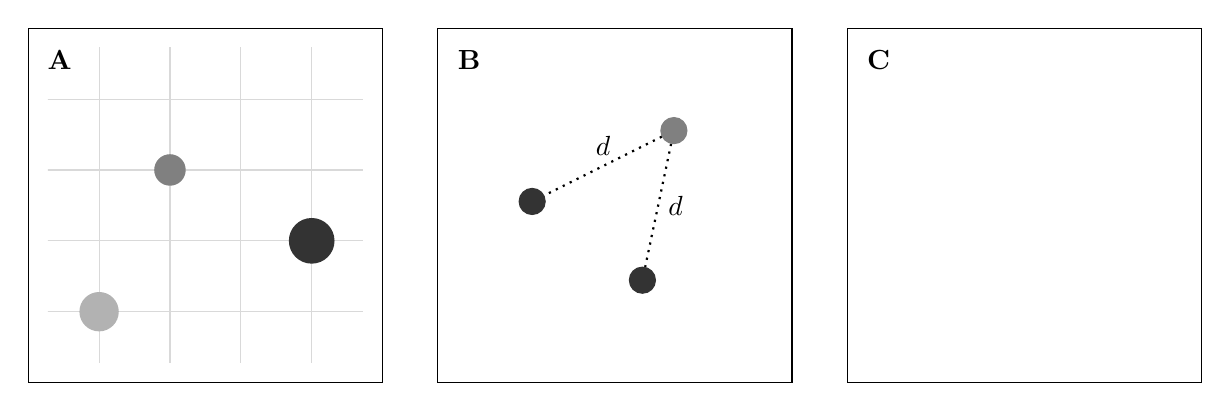
\begin{tikzpicture}[>=latex]
    \def\subwidth{4.5}
    \def\subheight{4.5}
    \def\spacing{0.7}

    \begin{scope}[shift={(0,0)}]
        \node at (0.4, \subheight - 0.4) {\textbf{A}};
        \begin{scope}
            \clip (0.25,0.25) rectangle (\subwidth-0.25, \subheight-0.25);
            \draw[step=0.9cm,gray!30,thin] (0,0) grid (\subwidth,\subheight);
            \fill[gray] (1.8,2.7) circle (0.2);
            \fill[black!80] (3.6,1.8) circle (0.29);
            \fill[black!30] (0.9,0.9) circle (0.25);
        \end{scope}
        \draw[thin] (0,0) rectangle (\subwidth, \subheight);
    \end{scope}

    \begin{scope}[shift={(\subwidth + \spacing, 0)}]
        \node at (0.4, \subheight - 0.4) {\textbf{B}};
        \node (c1) at (3.0,3.2) [draw,circle,fill,gray,radius=0.78] {};
        \node (c2) at (2.6,1.3) [draw,circle,fill,black!80,radius=0.8] {};
        \node (c3) at (1.2,2.3) [draw,circle,fill,black!80,radius=0.8] {};
        \draw[dotted,thick] (c1) -- node[right]{$d$} (c2);
        \draw[dotted,thick] (c1) -- node[above]{$d$} (c3);
        \draw[thin] (0,0) rectangle (\subwidth, \subheight);
    \end{scope}

    \begin{scope}[shift={(2*\subwidth + 2*\spacing, 0)}]
        \node at (0.4, \subheight - 0.4) {\textbf{C}};
        \draw[thin] (0,0) rectangle (\subwidth, \subheight);
    \end{scope}
\end{tikzpicture}
\end{document}
